 \documentclass[12pt, titlepage]{article}
 \usepackage{amsmath, empheq}
 \usepackage{amssymb}
 \usepackage{geometry}
 \geometry{
 	a4paper,
 	total={170mm,257mm},
 	left=20mm,
 	top=20mm,
 }
\usepackage[utf8]{inputenc}
\usepackage{graphicx}
\usepackage[font=small,labelfont=bf]{caption} % Required for specifying captions to tables and figures

\title{Práctica 2\\ 
\large Implementación del algoritmo del Simplex Primal }
\author{Pedro López Sancha, Emilia Vayssier}

\begin{document}
\maketitle

En este trabajo se ha implementado el algoritmo del Simplex Primal en dos lenguajes de programación distintos: C++ y MATLAB. \\
Se programaron dos versiones del algoritmo que difieren en la forma de elegir de la variable no básica de entrada a la base. La primera versión utiliza la Regla de Bland, mientras que la segunda utiliza la Regla del coste reducido más grande. Ambas versiones constan de las Fases I y II. \\
Se resolvieron los problemas planteados utilizando las dos versiones y se presenta una comparación del rendimiento. Los resultados vienen acompañados de la actualización de los valores a cada iteración.
\newpage
\section{Implementación en C++}
A pesar de que se recomendó emplear MATLAB como lenguaje de programación, hemos decidido implementar el algoritmo primeramente en C++ como divertimento, y también como práctica para otras asignaturas como Algoritmia.\\
Para ello, primeramente ha sido necesario crear una clase Matriz que permita trabajar con este tipo de objetos de manera cómoda. Posteriormente, tras depurar el código de la clase Matriz y tras una gran cantidad de pruebas, hemos conseguido desarrollar el Simplex primal, y hacer que este funcione correctamente.
\subsection{Clase Matriz}
La clase Matriz se ha implementado siguiendo el paradigma de la programación orientada a objetos. En esta sección se discutirán brevemente las funcionalidades básicas de la clase Matriz que se emplean en el algoritmo del Símplex.
\begin{itemize}
\item	La matriz internamente se guarda como un vector de vectores. Es por este motivo por el que se emplea el contenedor \textit{vector} de la librería estándar de C++. Esto además permite acceder al elemento $a_{ij}$ con una notación relativamente natural como es $matriz[i][j]$.
\item	Internamente se guardan las dimensiones de la matriz. Si en cualquier momento se accede a una posición que no pertenece a la matriz, las funciones de la clase devuelven $0$. 
\item	Las funciones que incorpora la clase Matriz para las operaciones básicas de matrices son:
\begin{itemize}
\item	Producto de una matriz por un escalar: \textit{scalarProduct} que recibe como parámetros una matriz y un escalar, y devuelve el producto de ambos.
\item	Suma de matrices: \textit{matrixSum} que recibe como parámetros dos matrices y devuelve su suma.
\item	Producto de matrices: \textit{matrixProduct} que recibe como parámetros dos matrices y devuelve su producto.
\item	Matriz transpuesta: \textit{transpose}, que recibe como parámetro una matriz y devuelve su transpuesta.
\item	Determinante: \textit{determinant} que recibe como parámetro una matriz y calcula el determinante usando menores. Cabe decir que es una manera ineficiente de calcularlo, por ello el tiempo de ejecución para matrices $10\times10$ como las proporcionadas en datos es del orden de 15 segundos. Por lo tanto, las funciones adjunta y inversa no se ejecutan para matrices grandes.
\item	Matriz adjunta:	\textit{adjoint}, que recibe como parámetro una matriz y devuelve su matriz de adjuntos.
\item	Matriz inversa:	\text{inverse}, que recibe como parámetro una matriz y calcula la inversa.
\end{itemize}
\item	Las funciones para la modificación de matrices son:
\begin{itemize}
\item	Inserción de fila y columna: \textit{insertRow} y \textit{insertCol}, que reciben como parámetros un vector de reales y la fila o columna en la cual se debe insertar.
\item	Inserción de matriz en fila y columna: \textit{insertMatrixInRow} y \textit{insertMatrixInCol}, que reciben como parámetros una matriz de las dimensiones adecuadas y la fila o columna en la cual se debe insertar.
\item	Reemplazo de fila y columna: \textit{replaceRow} y \textit{replaceCol}, que reciben como parámetros un vector y la fila o columna por la cual se debe reemplazar.
\item	Redondeo de matriz: \textit{roundMatrix}, que permite redondear todos los valores reales a su entero más cercano si están a una distancia de este inferior o igual a la suministrada como parámetro. Esta función es útil ya que en operaciones entre matrices grandes, el cálculo de números reales pierde precisión.
\end{itemize}
\item	Otras funciones relevantes son:
\begin{itemize}
\item	Matriz identidad: \textit{identity}, que retorna una matriz identidad de la dimensión dada.
\item	Información: \textit{info} y \textit{print}, que imprimen por pantalla información sobre el objeto.
\end{itemize}
\end{itemize}
\subsection{Implementación del Simplex Primal}
El algoritmo del símplex se ha implementado mediante dos archivos, el archivo de cabecera \textit{Simplex.h} que contiene las declaraciones de las funciones, y el archivo de implementación \textit{Simplex.cc}, que contiene las definiciones de dichas funciones. Se ha eligido esta metodología ya que es la recomendad por la comunidad de programación.\\

\subsubsection{Fases del Símplex}
Se han implementado las dos fases del Símplex, de modo que el programa recibe las matrices que representan el problema y este resuelve de manera autónoma la fase 1 y, si determina que es factible, continúa con la fase 2. Cada fase tiene su propia función, como se verá en el próximo apartado. Primeramente, mostramos brevemente las operaciones de cada fase:
\begin{itemize}
\item	Fase 1: primeramente, a partir de la matrices de coeficientes $A$, inserta la matriz identidad correspondiente a las variables artificiales de fase 1. También crea los vectores de coeficientes de la función objetivo de fase 1, así como el vector de variables básicas y no básicas. Por último, iguala la solución básica factible inicial $X_b$ al vector de términos independientes $b$ y calcula el valor de la función objetivo. A continuación, comienza a iterar el algoritmo. Una vez acaba, si el óptimo de la función objetivo es $z = 0$, o un valor cercano por error de aproximación, determina que el problema es factible. En tal caso, retorna la base óptima primal y su inversa. 
\item	Fase 2: a partir del vector de variables básicas y no básicas, crea los vectores de coeficientes de la función objetivo así como la matriz no básica $A_n$. Calcula el valor de la función objetivo en la base actual y, en lugar de calcular la inversa de la base, recibe la de fase 1. Seguidamente comienza a iterar el Símplex.
\end{itemize}
Ambas funciones tienen variables que determinan si estamos en el óptimo, si el problema es ilimitado o si es degenerado. El algoritmo itera mientras ninguna de estas condiciones se cumpla. En el momento que una de estas condiciones se da, para su ejecución y dice qué ha sucedido.
Las funciones se llaman desde el \textit{main} del programa. Entre las llamadas a ambas y, en caso de que el problema sea factible, se comprueba primeramente si han quedado variables artificiales en la base. En caso afirmativo, para la ejecución del programa. Si no, revisa el vector de variables no básicas y elimina aquellas que sean artificiales.

\subsubsection{Funciones en la implementación}
Cada paso del algoritmo tiene su propia función. De este modo, el código es más escalable, estructurado, legible y facilita la comprensión. Las funciones declaradas en el archivo de implementación són:
\begin{itemize}
\item	Cálculo de costes reducidos: \textit{computeReducedCosts}, que calcula el vector de costes reducidos. También determina si la solución básica factible actual es óptima, y en caso de que no lo sea, devuelve el índice $q$ de la variable no básica que debe entrar en la base y su posición en el vector de variables no básicas. En los argumentos de la función, se especifica si empleamos o no la regla de Bland y también en qué fase del Simplex estamos.
\item	Cálculo de la dirección básica factible: \textit{computeBasicFeasibleDirection}, que calcula la dirección básica factible en caso de que no estemos en el óptimo. También determina si nos encontramos ante un problema ilimitado buscando una componente negativa del vector.
\item	Cálculo de la longitud de paso: \textit{computeTheta}, que calcula la longitud de paso a lo largo de la dirección básica factible. Se ejecuta tan solo en caso de que el problema no sea ilimitado.
\item	Actualización de matrices:	\textit{updateMatrices}, que actualiza los vectores de coeficientes de variables básicas $c_b$ y no básicas $c_n$, la matriz $A_n$ de coeficientes de variables no básicas, y la inversa de la base $B^{-1}$. Esta última se calcula con la actualización de la inversa, en lugar de calcular la nueva matriz de base $B$ y posteriormente calcular la inversa.
\item	Actualización de variables:	\textit{updateVariables}, que actualiza la función objetivo, las componentes de la solución básica factible actual, y el vector de variables básicas y no básicas.
\item	Degeneración de la base: \textit{isDegenerate}, que busca alguna variable con valor $0$ en el vector la solución básica factible actual.
\item	Información: \textit{printIteration}, que imprime la información relevante sobre la última iteración.
\end{itemize}
\subsection{Errores de la implementación}
Como ya se ha mencionado anteriormente, en cálculos entre matrices de dimensiones del orden de $10 \times 10$, la pérdida de precisión en operaciones entre números reales es significativa. Por esta razón, a medida que el algoritmo itera, las matrices con las que opera se alejan más de las que deberían realmente ser. \\
A continuación se muestra un ejemplo que ilustra lo mencionado.\\
\begin{center}
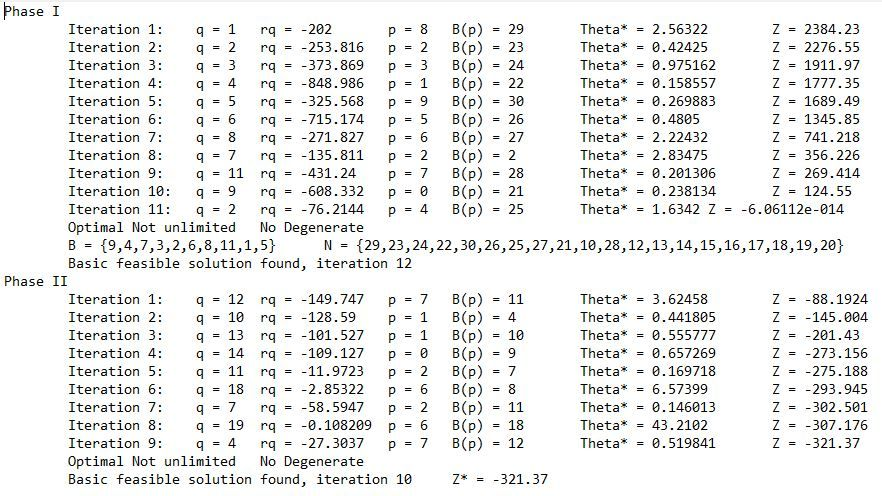
\includegraphics[scale=0.5]{imagenes/output_1_RB.JPG}
\captionof{figure}{problema 1 del conjunto 45 con regla de Bland}
\end{center}

\begin{center}
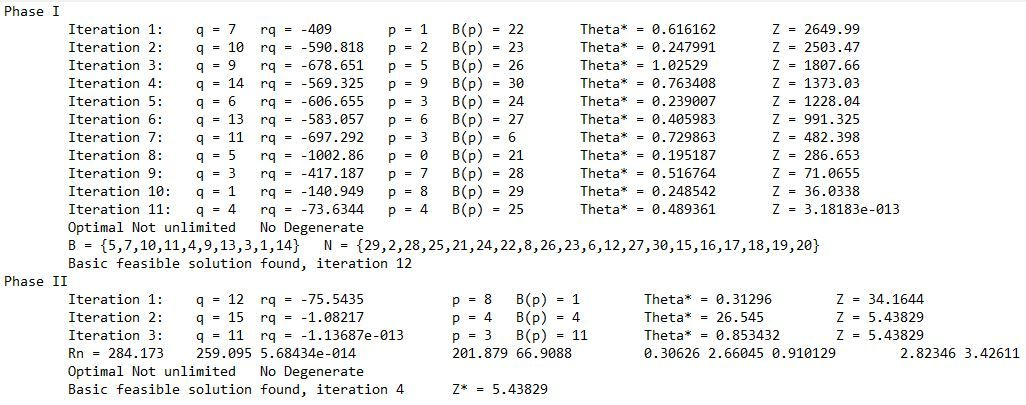
\includegraphics[scale=0.45]{imagenes/output_1_NRB.JPG}
\captionof{figure}{problema 1 del conjunto 45 con coste reducido más negativo}
\end{center}
Como se puede observar, aplicando regla de Bland el algoritmo da el mismo óptimo que la solución proporcionada en el conjunto de datos. Sin embargo, aplicando la regla del coste reducido más negativo, llega un momento en el que el vector de costes es no negativo y el algoritmo concluye que es óptimo. Como se puede ver, hay un valor muy cercano a cero, que podría ser negativo. En tal caso, el algoritmo habría seguido iterando.
\subsection{Posibles mejoras}
Como se ha mostrado, la implementación en C++ no funciona completamente, y creemos que es debido a los errores de cálculo que tiene el propio lenguaje. La solución a este problema está fuera de nuestros alcance. No obstante, en caso de descubrir o implementar una librería que esté libre de este tipo de errores, podríamos incluir las siguientes mejoras:
\begin{itemize}
\item	En caso de que encuentre degeneración y de estar usando la regla del coste reducido más negativo, no parar la ejecución del algoritmo, sino crear una lista con todas las bases por las que el algoritmo ha pasado a partir de la detección de degeneración. Así, tras cada iteración, podríamos comprobar si la base actual ya ha sido visitada. En caso afirmativo, probablemente indicaría que el Símplex está ciclando, y por tanto el algoritmo no asegura su convergencia.
\end{itemize}
\newpage
\section{Implementación en MATLAB}
	
\end{document}